\chapter{Background \& Related Work}

\section{Background}

\subsection{Lead Sheets}

Lead sheets are a form of musical notation that contain both the melody and harmony. Generally, the melody is a single line forming the dominant melody, which is often the vocal line of a song, written in standard musical notation on a stave. The harmony is represented by chord symbols, which are written above the melody. A lead sheet also contains the key, time signature and, optionally, the lyrics of a song. An example of a lead sheet is shown in Figure~\ref{fig:lead_sheet_example}.


\begin{figure}[h]
    \centering
    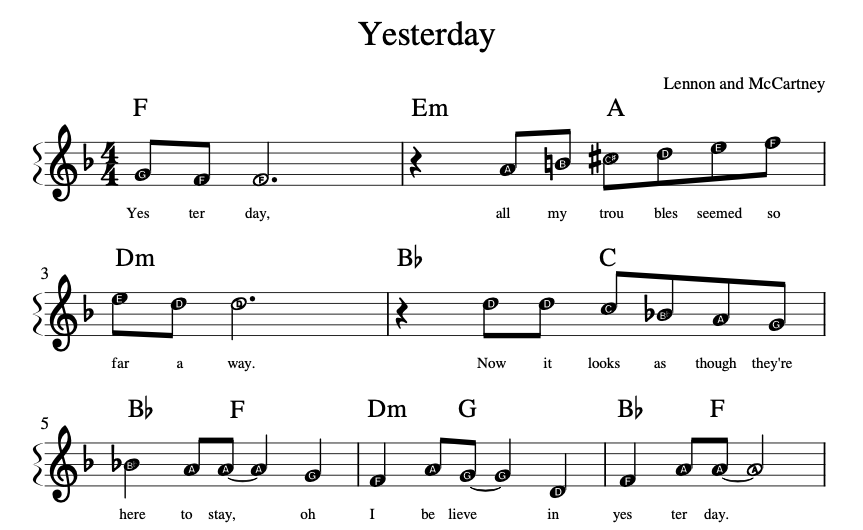
\includegraphics[width=0.8\textwidth]{images/lead_sheet_example.png}
    \caption{An example of a lead sheet for `Yesterday' by the Beatles.}
    \label{fig:lead_sheet_example}
\end{figure}

They date back to the mid 20th century, and were originally called `fake sheets' because they were used by musicians to `fake' their way through a song~\cite{RealBookPodcast}. Lead sheets are most notably used in jazz music where their origins lie. Any jazz musician worth their salt owns a `real book', so called to distinguish it from the fake books that were used in the past. Real books contain lead sheets for hundreds of jazz standards, and are an essential tool for any jazz musician. 

More recently they have served as a useful tool for musicians in other genres, such as pop and rock, who want to learn and perform songs quickly and easily. They allow easy communication of the important elements of a song, without the need for a full score, further allowing improvisation and personalisation of the song.

Lead sheets do not contain all the information of a full score, such as dynamics, articulation, or specific voicings of chords. Furthermore, they are not suitable for all types of music, such as classical music, where a full score is necessary to convey the composer's intentions, or rap music where the lyrics and beat are the most important elements. However, they are a useful tool for many musicians, and are a common way of representing music in the music industry.

\subsection{Music Transcription}

Musical Transcription is a field within MIR (Music Information Retrieval) that aims to convert audio into a symbolic representation.~\cite{ComprehensiveReviewMusicTranscription} provides a comprehensive review of different forms of transcription. They categorise transcription into frame-level, note-level, stream-level and notation-level transcription. In brief, frame-level transcription predicts musical features, such as pitch, for a short frame of audio, which can then be aggregated into note-level predictions for musical notes. Stream-level transcription involves looking at the large picture of a piece of music such as phrasing and structure, and notation level then assembles all of this information into a human-readable score.

For lead sheet transcription, we are interested in this highest level of transcription. We want to take an audio recording of a song and generate a lead sheet that contains the melody and harmony of the song. This is a challenging task, as it requires the model to isolate and transcribe a melody, transcribe the chordal information, and then combine these two elements into a coherent lead sheet where the melody and harmony are aligned in time/beat.

\subsection{Music Features}

Brief explanation of CQT and chroma vectors. GPT generated features~\cite{MelodyTranscriptionViaGenerativePreTraining}.

\section{Related Work}

\subsection{Lead Sheet Transcription}

~\cite{MelodyTranscriptionViaGenerativePreTraining} is the only work I've found that does specific lead shet generation. However, they focused far more on melody transcription, and their model is only effective for 24s of audio. They also do not transcribe the lyrics. They also trained on HookTheory user-submitted data which is not ideal - perhaps biased to simpler transcriptions? This work uses well known, expert datasets.

They proposed the use of a generative pre-trained transformer to provide the features, rather than traditionally used CQT features.

\subsection{Automatic Chord Recognition}

JAAH,

Datasets: Isophonics, Mcgill, RWC, USPop, HookTheory

Evaluation: MIREX standard evaluation. Confusion matrices for chords. Qualitative evaluation.

Suffer from lack of variety and size, and distribution of chords. Attempted remedy by~\cite{BalanceACRRandomForests}.

\subsection{Melody Transcription}

Transformer SOTA. 

Datasets: MAPS, MDB, MedleyDB, WJazzD, RWC, USPop, HookTheory

Evaluation: MIREX standard evaluation. F1 scores, precision, recall. Qualitative evaluation.

\subsection{Data Scarcity}

Resampling: ~\cite{BalanceACRRandomForests}
Augmentation:
Semi-supervised learning
Synthetic data gen:

\subsection{Music Generation}

Jukebox~\cite{Jukebox}

Music generation for MIR:~\cite{MusicGenTrainingData}